\section{Pipeline metodologica generale} \label{chap:pipeline}

Il presente lavoro adotta una pipeline metodologica strutturata, orientata alla valutazione della robustezza operativa di strumenti forensi basati su intelligenza artificiale (AI) quando sottoposti a perturbazioni avversariali e anti-forensi. Tale pipeline è stata disegnata con l'obiettivo di simulare uno scenario realistico, in cui i modelli di classificazione automatica integrati nei software analizzati operano su immagini raccolte da fonti eterogenee e potenzialmente ostili.

\textbf{La scelta della sequenza metodologica non è casuale:} essa è motivata dal desiderio di replicare, seppur in ambiente controllato, le condizioni tipiche delle indagini digitali contemporanee, nelle quali i sistemi automatici devono fronteggiare input non certificati, manipolabili e potenzialmente malevoli. La struttura segue le raccomandazioni emerse nella recente letteratura sulla sicurezza dei modelli AI in contesti forensi~\cite{barni2020forensics, nowroozi2020presentation, costantini2019digital}.

La pipeline si articola nei seguenti passaggi principali, ciascuno dei quali è approfondito nei capitoli successivi:

\begin{enumerate}
    \item \textbf{Definizione del contesto sperimentale}: identificazione del dominio forense di interesse (in questo caso, la classificazione automatizzata di armi da fuoco in immagini digitali) e selezione degli strumenti AI-based oggetto di valutazione, tra cui \textit{Magnet Axiom}, \textit{UFED}, \textit{X-Ways Forensics} e \textit{Oxygen Forensics}. \textit{(Si veda Capitolo~\ref{chap:strumenti})}
    
    \item \textbf{Costruzione di dataset realistici}: creazione di un corpus bilanciato e rappresentativo di immagini da cinque fonti distinte (dataset pubblici, scraping web, Telegram, YouTube e deep web), al fine di riflettere la varietà semantica e visiva presente nei contesti investigativi reali. \textit{(Approfondito in Capitolo~\ref{chap:dataset})}
    
    \item \textbf{Preprocessing e validazione del dataset}: rimozione di immagini corrotte, normalizzazione dimensionale e verifica qualitativa/manuale per assicurare la coerenza delle etichette e la pertinenza tematica rispetto al dominio d’interesse.
    
    \item \textbf{Applicazione di perturbazioni controllate}: ciascuna immagine è sottoposta a trasformazioni controllate, mediante tecniche di attacco suddivise tra:
    \begin{itemize}
        \item \textit{Adversarial attacks} (es. FGSM, DeepFool, One Pixel Attack, SuperDeepFool);
        \item \textit{Tecniche anti-forensi} (es. color shifting, JPEG compression, Gaussian blur, occlusion patch).
    \end{itemize}
    Tali tecniche sono state selezionate in base alla letteratura sul tema della sicurezza dei modelli AI e della counter-forensics~\cite{barni2020forensics, nowroozi2020presentation}.
    
    \item \textbf{Valutazione empirica}: le immagini originali e quelle perturbate vengono sottoposte agli strumenti AI-based in analisi, registrando l’accuratezza delle classificazioni effettuate, la stabilità dei risultati e l'eventuale presenza di errori sistematici.
    
    \item \textbf{Analisi qualitativa}: studio dei casi di errore significativi, con particolare attenzione agli input OOD (\textit{out-of-distribution}) e ai fallimenti specifici dei modelli, al fine di comprendere le dinamiche di degrado decisionale. \textit{(Discussione completa in Capitolo~\ref{chap:discussion})}
\end{enumerate}

Questa pipeline riflette l'approccio \textit{adversary-aware} suggerito dalla recente letteratura in ambito di forensics e sicurezza del machine learning~\cite{costantini2019digital}, e si propone di offrire una valutazione integrata, tecnica e sperimentalmente fondata, sull'efficacia degli strumenti AI-based quando operano in contesti realisticamente ostili.

\subsection*{Limitazioni della pipeline}

Sebbene la pipeline proposta sia stata progettata per simulare in modo realistico uno scenario operativo forense, essa presenta alcune limitazioni intrinseche. In particolare, l'analisi è stata condotta su un numero finito di immagini, che sebbene eterogenee, non può rappresentare l'intera varietà del dominio visivo forense. Inoltre, gli strumenti AI-based testati sono spesso sistemi chiusi (black-box), limitando l'accesso diretto alla struttura interna del modello e alla spiegabilità dei risultati.

Un'ulteriore limitazione riguarda la selezione delle tecniche di perturbazione: nonostante si sia fatto riferimento a metodologie consolidate in letteratura, non è possibile escludere che attacchi più sofisticati o combinazioni di tecniche non ancora note possano produrre risultati differenti. Infine, l'assenza di una ground truth ufficiale di riferimento limita la possibilità di calcolare metriche di errore assoluto.

\subsection*{Schema della pipeline decisionale}

\begin{figure}[H]
\centering
\begin{tikzpicture}[node distance=1.6cm and 3.5cm, every node/.style={align=center}, scale=0.92, transform shape]
\tikzstyle{block} = [rectangle, draw=black, fill=blue!10, rounded corners, text width=5.3cm, minimum height=1.2cm, text centered, font=\footnotesize\bfseries]
\tikzstyle{arrow} = [->, thick]

\node (input) [block] {Acquisizione immagini da 5 dataset realistici};
\node (check) [block, below=of input] {Validazione manuale e preprocessing};
\node (perturb) [block, below=of check] {Applicazione di perturbazioni controllate};
\node (tool) [block, below=of perturb] {Classificazione tramite strumenti forensi AI-based};
\node (eval) [block, below=of tool] {Valutazione risultati (accuratezza, stabilità)};
\node (analysis) [block, below=of eval] {Analisi qualitativa e casi critici};

% arrows
\draw[arrow] (input) -- (check);
\draw[arrow] (check) -- (perturb);
\draw[arrow] (perturb) -- (tool);
\draw[arrow] (tool) -- (eval);
\draw[arrow] (eval) -- (analysis);

\end{tikzpicture}
\caption{Flusso decisionale della pipeline sperimentale adottata}
\label{fig:flow_pipeline}
\end{figure}



\section{Metodologia sperimentale}
\label{sec:metodologia}

Lo scopo di questa fase è valutare la robustezza operativa di strumenti forensi AI-based, in condizioni realistiche ma controllate. La pipeline sperimentale adottata si articola in sei fasi principali, riportate nella Figura~\ref{fig:experimental-pipeline}.

\begin{figure}[H]
  \centering
  \begin{tikzpicture}[node distance=1.8cm and 1.6cm, font=\small]
  \tikzset{  arrow/.style={->,>=Stealth,thick}}

  % Nodi
  \node (acquisition) [block] {1. Acquisizione immagini\\ (5 dataset da 200 immagini)};
  \node (validation)  [block, below=of acquisition] {2. Validazione automatica\\ (qualità, dimensioni, duplicati)};
  \node (split)       [block, below=of validation]  {3. Suddivisione bilanciata\\ (5 subset da 200 immagini)};
  \node (ood)         [block, below=of split]       {4. Rilevamento OOD\\ (CLIP + annotazione manuale)};
  \node (bias)        [block, below=of ood]         {5. Analisi esplorativa dei bias\\ (fonte, semantica, qualità)};
  \node (attack)      [block, below=of bias]        {6. Generazione attacchi\\ (FGSM, JPEG, SuperDeepFool, ecc.)};

  % Frecce
  \draw [arrow] (acquisition) -- (validation);
  \draw [arrow] (validation) -- (split);
  \draw [arrow] (split) -- (ood);
  \draw [arrow] (ood) -- (bias);
  \draw [arrow] (bias) -- (attack);

  \end{tikzpicture}
  \caption{Pipeline sperimentale: dalla raccolta dati alla valutazione della robustezza dei modelli AI.}
  \label{fig:experimental-pipeline}
\end{figure}

Ciascuna fase sarà descritta in dettaglio nelle sezioni successive.




\section{Analisi della distribuzione e valutazione di bias nei sottoinsiemi di test}
\label{sec:dataset-bias}

Per valutare la robustezza e l’affidabilità dei modelli AI-based nel contesto forense, è stata condotta un’analisi strutturata sui dati utilizzati, con particolare attenzione alla possibile presenza di \textbf{bias sistematici}. In scenari investigativi reali, la presenza di bias nei dataset o nei modelli può compromettere la correttezza delle inferenze, portando a errori critici come l'omissione o la sovrastima di evidenze digitali.





\subsection{Analisi esplorativa dei bias}
\label{subsec:exploratory-bias}

Al fine di indagare l’eventuale presenza di bias nei modelli AI-based utilizzati per la classificazione forense, è stata condotta un’analisi mirata basata sulla suddivisione controllata del dataset sperimentale.

Partendo da un insieme di \textbf{1000 immagini annotate manualmente} come \texttt{ARMA} o \texttt{NON ARMA}, si è proceduto alla creazione di \textbf{5 sottoinsiemi bilanciati}, ciascuno composto da 200 immagini. La suddivisione è stata effettuata tramite uno \textit{Stratified K-Fold} (con \texttt{n\_splits=5}), al fine di mantenere la proporzione originale tra le due classi in ogni subset. Questo approccio consente di verificare in modo più robusto la coerenza predittiva dei modelli, riducendo l’impatto di fluttuazioni casuali legate alla selezione dei dati.

\medskip

L’obiettivo dell’analisi è stato quello di valutare:

\begin{itemize}
  \item se alcune tipologie di immagini (es. da deep web o Telegram) siano associate a un numero più elevato di errori;
  \item se l’accuratezza dei modelli vari al variare del contesto visivo (es. sfondo reale vs neutro, risoluzione, qualità);
  \item se vi siano differenze significative nei tassi di disaccordo tra la classificazione automatica (es. CLIP) e l’annotazione umana.
\end{itemize}

I criteri di segmentazione e confronto includono:

\begin{itemize}
  \item \textbf{Fonte del dataset}: ogni immagine mantiene il riferimento alla sorgente originale (es. Kaggle, YouTube, Telegram, Deep Web);
  \item \textbf{Tipo semantico}: immagini ambientate nel contesto reale vs oggetti su sfondo neutro;
  \item \textbf{Qualità visiva}: nitide vs sfocate, alta vs bassa risoluzione;
  \item \textbf{Classe oggetto}, ove disponibile: handgun, rifle, ecc.
\end{itemize}

\medskip

Le metriche calcolate su ciascun sottoinsieme includono:

\begin{itemize}
  \item \textbf{Accuracy}, \textbf{Precision}, \textbf{Recall} (sia del modello CLIP che rispetto all’etichettatura manuale);
  \item \textbf{Distribuzione delle immagini OOD} secondo CLIP e secondo l’annotazione dell’operatore;
  \item \textbf{Tasso di disaccordo} tra le due etichette;
  \item \textbf{Percentuale di immagini ambigue} (es. un’arma classificata come OOD o viceversa).
\end{itemize}

\begin{figure}[H]
\centering
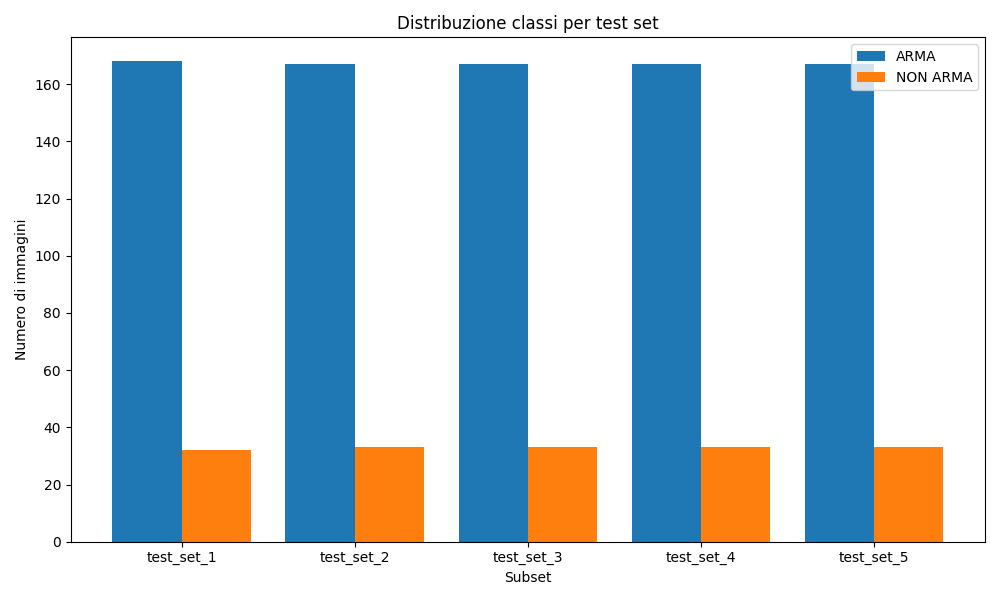
\includegraphics[width=0.8\textwidth]{images/class_distribution_plot.png}
\caption{Distribuzione delle classi ARMA e NON ARMA nei 5 test set bilanciati.}
\label{fig:class-distribution}
\end{figure}

Questa analisi si è rivelata essenziale per evidenziare eventuali bias sistematici nei modelli AI impiegati, fornendo una base di partenza oggettiva per la successiva valutazione della loro resilienza agli attacchi adversariali.



\subsection{Stratified K-Fold: principio e applicazione}
Per garantire che ogni sottoinsieme di test mantenga la stessa distribuzione tra le classi \texttt{ARMA} e \texttt{NON ARMA} del dataset complessivo, è stato utilizzato lo \textbf{Stratified K-Fold Cross-Validation}, una tecnica comunemente adottata in ambito di valutazione statistica dei modelli di classificazione~\cite{scikit-learn}.

A differenza del semplice \textit{K-Fold}, che suddivide il dataset in $K$ blocchi di pari dimensione ignorando la distribuzione delle classi, lo \textit{Stratified K-Fold} preserva la proporzione tra le classi all’interno di ciascun fold. Questo è particolarmente utile in presenza di dataset sbilanciati o in compiti binari, come nel caso della presente tesi, in cui è fondamentale mantenere un equilibrio costante tra immagini contenenti armi reali e immagini prive di armi.

Nel nostro caso, è stato impostato un valore di $K=5$, ottenendo così cinque subset da 200 immagini ciascuno, con distribuzione di classe bilanciata come mostrato nella Tabella~\ref{tab:class-dist}. Questo approccio ha garantito una valutazione più robusta e statisticamente affidabile delle performance dei classificatori.






\subsection{Suddivisione del dataset in test set bilanciati}
\label{subsec:balanced-testset}

In coerenza con la metodologia descritta in~\cite{phd_unisi_068552, nowroozi2020adversarial, s10472-019-09632-y}, il dataset è stato suddiviso in \textbf{5 sottoinsiemi bilanciati}, mantenendo proporzioni costanti tra le classi \texttt{ARMA} e \texttt{NON ARMA} (etichettate tramite annotazione manuale).

Questa strategia di \textit{stratified splitting} permette di:

\begin{itemize}
  \item testare i modelli in condizioni statisticamente equivalenti ma visivamente variabili;
  \item valutare la stabilità delle predizioni su diversi sample;
  \item evidenziare possibili pattern sistematici di errore.
\end{itemize}

I dettagli di distribuzione delle classi nei subset sono riportati nella Tabella~\ref{tab:class-dist}.

\begin{table}[H]
\centering
\begin{tabular}{lcccc}
\toprule
\textbf{Subset} & \textbf{Totale} & \textbf{ARMA} & \textbf{NON ARMA} & \textbf{\% ARMA} \\
\midrule
test\_set\_1 & 200 & 175 & 25 & 87.5\% \\
test\_set\_2 & 200 & 175 & 25 & 87.5\% \\
test\_set\_3 & 200 & 175 & 25 & 87.5\% \\
test\_set\_4 & 200 & 174 & 26 & 87.0\% \\
test\_set\_5 & 200 & 174 & 26 & 87.0\% \\
\bottomrule
\end{tabular}
\caption{Distribuzione delle classi nei subset bilanciati generati.}
\label{tab:class-dist}
\end{table}

I grafici generati (Appendice~\ref{appendix:testset-plots}) mostrano visivamente l'equilibrio raggiunto, sia in valore assoluto che in percentuale, tramite:
\begin{itemize}
  \item barre affiancate (`barre\_affiancate.png`);
  \item barre sovrapposte (`barre\_stacked.png`);
  \item grafici percentuali (`barre\_percentuali.png`).
\end{itemize}

\subsection{Considerazioni operative}
L’identificazione di bias e l’uso di subset bilanciati rappresentano un passo fondamentale per un utilizzo forense affidabile dell’intelligenza artificiale. In assenza di tale analisi, un errore di classificazione dovuto a fattori ambientali o qualitativi potrebbe compromettere l'integrità dell'intera catena investigativa.



\paragraph{Collegamento con la fase di costruzione del dataset}
L’analisi esplorativa dei bias descritta in questa sezione si fonda direttamente sulla struttura bilanciata e multi-sorgente del dataset costruito nella Sezione~\ref{sec:dataset-selection}. La varietà semantica e visiva delle immagini selezionate, unita ai controlli di qualità e validazione automatica, costituisce un prerequisito essenziale per la valutazione comparativa dei modelli AI-based in contesti realistici e operativi.




\section{Confronto tra modelli di classificazione automatica}
\label{sec:confronto-modelli}

Nel contesto della classificazione automatizzata di immagini in ambito forense, sono stati impiegati e confrontati quattro approcci distinti, rappresentativi di diverse filosofie di progettazione e addestramento dei modelli di visione artificiale. La tabella~\ref{tab:confronto-modelli} ne sintetizza le principali caratteristiche.

\begin{itemize}
    \item \textbf{CLIP (Contrastive Language–Image Pre-training)}: modello multimodale sviluppato da OpenAI, pre-addestrato su una vasta collezione di coppie immagine-testo. CLIP apprende una rappresentazione condivisa per linguaggio naturale e immagini, ed è in grado di effettuare classificazioni zero-shot utilizzando prompt testuali descrittivi. Questa capacità lo rende particolarmente adatto a contesti open-world e non supervisionati.

    \item \textbf{BLIP (Bootstrapping Language-Image Pre-training)}: modello multimodale di seconda generazione, in grado di generare caption descrittive e apprendere rappresentazioni semantiche più profonde rispetto a CLIP. A differenza di CLIP, BLIP è ottimizzato anche per il \textit{visual question answering} e la generazione automatica di descrizioni, offrendo un approccio più descrittivo alla classificazione.

    \item \textbf{ResNet18 + SVM}: architettura classica supervisionata, composta da una rete convoluzionale ResNet18 (pre-addestrata su ImageNet) utilizzata come estrattore di feature, seguita da un classificatore SVM addestrato manualmente su un sottoinsieme del dataset finale. Questo approccio rappresenta una pipeline \textit{feature-based}, che disaccoppia l’estrazione dalla classificazione, risultando utile in scenari controllati.

    \item \textbf{CNN supervisionata (EfficientNet-B0)}: architettura CNN moderna, addestrata end-to-end su un dataset supervisionato contenente immagini etichettate come “arma” o “non arma”. EfficientNet-B0 offre un buon compromesso tra accuratezza e complessità computazionale, ed è spesso impiegata come baseline in esperimenti di classificazione robusta.
\end{itemize}

\begin{table}[H]
\centering
\caption{Confronto tra modelli utilizzati per la classificazione automatica}
\label{tab:confronto-modelli}
\begin{tabularx}{\textwidth}{|l|X|X|}
\hline
\textbf{Modello} & \textbf{Tipo} & \textbf{Caratteristiche principali} \\
\hline
CLIP & Pre-addestrato multimodale & Zero-shot, classificazione tramite prompt testuali, robusto al dominio, nessun fine-tuning necessario \\
\hline
BLIP & Pre-addestrato multimodale & Caption generation, VQA, inferenza semantica approfondita, descrizione libera delle immagini \\
\hline
ResNet18 + SVM & Supervisionato (feature-based) & Estrattore di feature + classificatore SVM, richiede etichette, sensibile a variazioni del dominio \\
\hline
EfficientNet-B0 & Supervisionato (end-to-end) & Addestramento completo sul dataset target, elevata accuratezza, adatto a contesto chiuso \\
\hline
\end{tabularx}
\end{table}

Questa eterogeneità di approcci consente una valutazione più ampia e realistica della robustezza dei sistemi AI in ambito forense, soprattutto in scenari in cui le immagini possono essere manipolate, ambigue o fuori distribuzione (OOD).



\subsection*{Conclusione}

Questa pipeline costituisce il nucleo operativo dell’intera tesi, fornendo un quadro metodologico rigoroso e riproducibile per l’analisi della robustezza degli strumenti AI-based applicati alla classificazione forense di immagini. L'integrazione di perturbazioni realistiche, provenienza eterogenea delle immagini e strumenti effettivamente usati nella pratica investigativa rappresenta un importante passo avanti rispetto a molti studi precedenti, spesso basati su scenari sintetici o idealizzati. I risultati ottenuti attraverso questa pipeline sono discussi nei capitoli successivi, con particolare attenzione alle vulnerabilità evidenziate e alle implicazioni per il futuro della digital forensics assistita da intelligenza artificiale.






